\documentclass[14pt,usepdftitle=false,aspectratio=169]{beamer}
\usepackage{preambule}
\setbeamercolor{structure}{fg=black}
\newcommand\N{\mathbb{N}}\newcommand\R{\mathbb{R}}\let\oldlim\lim\renewcommand\lim[2]{\oldlim\limits_{#1}\l#2\r}\let\oldexp\exp\renewcommand\exp[2][]{\oldexp^{#1}\l#2\r}\let\oldln\ln\renewcommand\ln[2][]{\oldln^{#1}\l#2\r}\usepackage{graphs}\usepackage{trigo}\usepackage{mathtools}\usepackage{tables}\usepackage{rotating}\usepackage{analyse}
\hypersetup{pdftitle=Analyse -- Fonctions usuelles}
\title{Analyse\\\emph{Fonctions usuelles}}
\author{}
\date{}
\begin{document}
\begin{frame}
    \titlepage
\end{frame}
\slideq{$\lim{x\to+\infty}{\th{x}}$}{1/55}
\slider{$1$}{1/55}
\slideq{Courbe représentative de $\ln{x}$}{2/55}
\slider{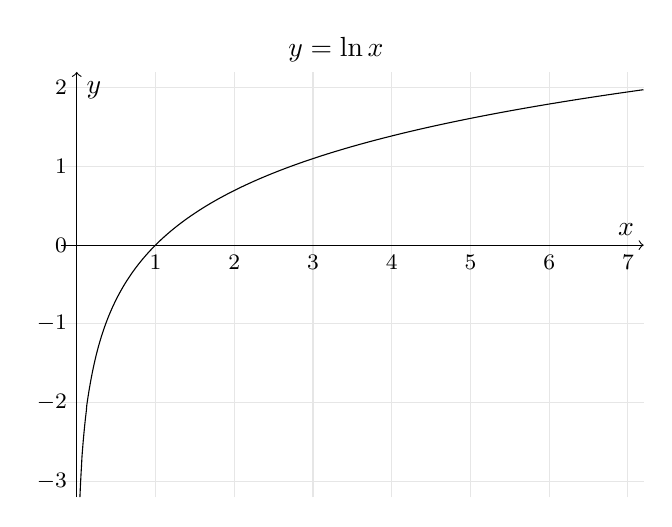
\begin{tikzpicture}\draw[color=gray,opacity=0.2] (-0.2,-3.2) grid(7.2,2.2); \draw[->] (0, -3.2) -- (0, 2.2) node[below right]{$y$}; \draw[->] (-0.2, 0) -- (7.2, 0) node[above left]{$x$}; \foreach \x in {1,...,7} \draw(\x,0) node[below]{\footnotesize$\x$}; \foreach \y in {-3,...,2} \draw(0,\y) node[left]{\footnotesize$\y$}; \draw[domain=0.0405:7.2, samples=1400, scale=1, smooth, variable=\x, black] plot (\x,{ln(\x)}); \node[above] at (current bounding box.north) {$y=\ln{x}$}; \end{tikzpicture}}{2/55}
\slideq{Propriétés remarquables de $\acos{x}$}{3/55}
\slider{$\forall x\in\left[-1,1\right],\;\cos{\acos{x}}=x$\linebreak$\forall x\in\left[0,\pi\right],\;\acos{\cos{x}}=x$\linebreak$\forall x\in\left[-\pi,0\right],\;\acos{\cos{x}}=-x$}{3/55}
\slideq{Expression de $\ath{x}$}{4/55}
\slider{$\frac{1}{2}\ln{\frac{1+x}{1-x}}=\ln{\sqrt{\frac{1+x}{1-x}}}$}{4/55}
\slideq{$\der{\th{x}}$}{5/55}
\slider{$1-\th[2]{x}=\frac{1}{\ch[2]{x}}$}{5/55}
\slideq{$\lim{x\to0}{\frac{\th{x}}{x}}$}{6/55}
\slider{$1$}{6/55}
\slideq{Courbe représentative de $\sh{x}$}{7/55}
\slider{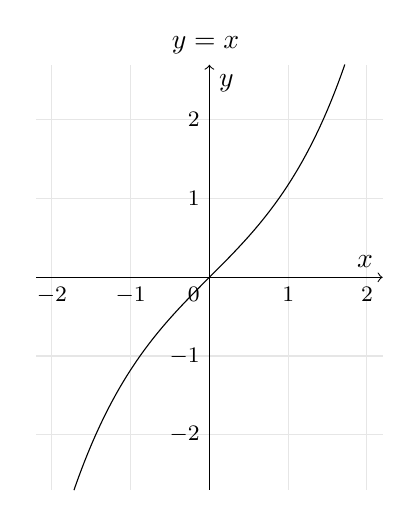
\begin{tikzpicture} \draw[color=gray,opacity=0.2] (-2.2,-2.7) grid (2.2,2.7); \draw[->] (-2.2, 0) -- (2.2, 0) node[above left]{$x$}; \draw[->] (0,-2.7) -- (0, 2.7) node[below right]{$y$}; \foreach \y in {-2,-1,1,2} \draw(0,\y) node[left]{\footnotesize$\y$}; \foreach \x in {-2,-1} \draw(\x,0) node[below]{\footnotesize$\x$}; \foreach \x in {1,2} \draw(\x,0) node[below]{\footnotesize$\x$}; \draw(0,0) node[below left]{\footnotesize$0$}; \draw[domain=-1.72:1.72, samples=400, scale=1, smooth, variable=\x, black] plot (\x,{(exp(\x)-exp(-\x))/2}); \node[above] at (current bounding box.north) {$y=\sh{x}$}; \end{tikzpicture}}{7/55}
\slideq{$\lim{x\to0}{\frac{\ln{1-x}}{x}}$}{8/55}
\slider{1}{8/55}
\slideq{$\der{\acos{x}}$}{9/55}
\slider{$-\frac{1}{\sqrt{1-x^2}}$}{9/55}
\slideq{Inégalité classique de $\atan{x}$}{10/55}
\slider{$\forall x\in\R,\;\left|\atan{x}\right|\leqslant\left|x\right|$}{10/55}
\slideq{Argument d'un nombre complexe $z$ avec $\atan{x}$}{11/55}
\slider{$\arg\l z\r\equiv\atan{\frac{\Im\l z\r}{\Re\l z\r}}\,\left[\pi\right]$}{11/55}
\slideq{Expression de $\ach{x}$}{12/55}
\slider{$\ln{x+\sqrt{x^2-1}}$}{12/55}
\slideq{Courbe représentative de $\ash{x}$}{13/55}
\slider{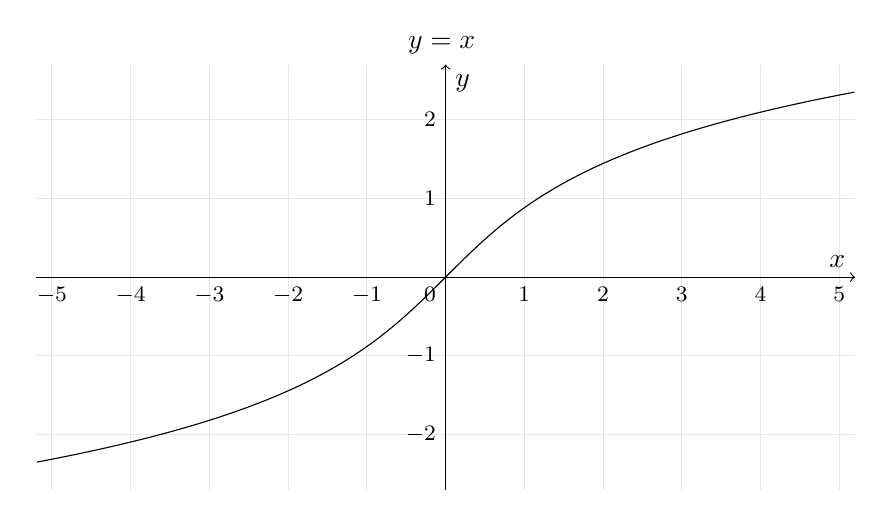
\begin{tikzpicture} \draw[color=gray,opacity=0.2] (-5.2,-2.7) grid (5.2,2.7); \draw[->] (-5.2, 0) -- (5.2, 0) node[above left]{$x$}; \draw[->] (0,-2.7) -- (0, 2.7) node[below right]{$y$}; \foreach \y in {-2,-1,1,2} \draw(0,\y) node[left]{\footnotesize$\y$}; \foreach \x in {-5,...,-1} \draw(\x,0) node[below]{\footnotesize$\x$}; \foreach \x in {1,...,5} \draw(\x,0) node[below]{\footnotesize$\x$}; \draw(0,0) node[below left]{\footnotesize$0$}; \draw[domain=0:5.2, samples=600, scale=1, smooth, variable=\x, black] plot (\x,{ln(\x+sqrt(\x*\x+1))}); \draw[domain=0:5.2, samples=600, scale=1, smooth, variable=\x, black] plot (-\x,{-ln(\x+sqrt(\x*\x+1))}); \node[above] at (current bounding box.north) {$y=\ash{x}$}; \end{tikzpicture}}{13/55}
\slideq{$n\in\N^*$, $x\in\R$\linebreak$\der[n]{\exp{x}}$}{14/55}
\slider{$\exp{x}$}{14/55}
\slideq{$n\in\N^*$, $x\in\R$\linebreak$\der[n]{\cos{x}}$}{15/55}
\slider{$\cos{x+\frac{n\pi}{2}}=\left\{\begin{matrix*}[l]\l-1\r^{\left\lfloor\oldfrac{n}{2}\right\rfloor}\cos{x}&\;\text{si }n\in2\N\\\l-1\r^{\left\lfloor\oldfrac{n}{2}\right\rfloor+1}\sin{x}&\;\text{sinon}\end{matrix*}\right.\!$}{15/55}
\slideq{Valeurs remarquables de $\asin{x}$ et $\acos{x}$}{16/55}
\slider{\setcolrow{6}{3}\begin{tikzpicture}[ampersand replacement=\&] \matrix (mat) [table] {  \&$0$\&$\oldfrac{1}{2}$\&$\oldfrac{\sqrt{2}}{2}$\&$\oldfrac{\sqrt{3}}{2}$\&$1$\\ \begin{turn}{45}$\arcsin$\end{turn}\&$0$\&$\oldfrac{\pi}{6}$\&$\oldfrac{\pi}{4}$\&$\oldfrac{\pi}{3}$\&$\oldfrac{\pi}{2}$\\ \begin{turn}{45}$\arccos$\end{turn}\&$\oldfrac{\pi}{2}$\&$\oldfrac{\pi}{3}$\&$\oldfrac{\pi}{4}$\&$\oldfrac{\pi}{6}$\&$0$\\ }; \draw [line width=0.5mm] (-10cm/3,-6.5cm/2) -- (-10cm/3,6.5cm/2); \draw [line width=0.5mm] (-10cm/2,6.5cm/6) -- (10cm/2,6.5cm/6); \draw [line width=0.5mm] (-5cm,-3.25cm) rectangle (5cm,3.25cm); \end{tikzpicture}}{16/55}
\slideq{$n\in\N^*$, $x\in\R$\linebreak$\der[n]{\sh{x}}$}{17/55}
\slider{$\left\{\begin{matrix*}[l]\sh{x}&\;\text{si }n\in2\N\\\ch{x}&\;\text{sinon}\end{matrix*}\right.\!$}{17/55}
\slideq{Expression de $\ash{x}$}{18/55}
\slider{$\ln{x+\sqrt{x^2+1}}$}{18/55}
\slideq{Courbe représentative de $\asin{x}$}{19/55}
\slider{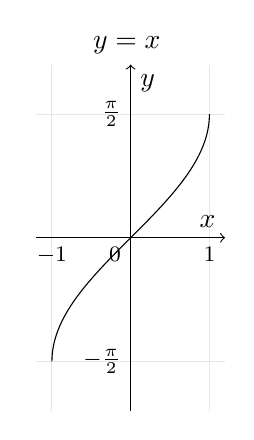
\begin{tikzpicture} \draw[color=gray,opacity=0.2] (-1.2,-2.2) grid[ystep=pi/2](1.2,2.2); \draw[->] (-1.2, 0) -- (1.2, 0) node[above left]{$x$}; \draw[->] (0,-2.2) -- (0, 2.2) node[below right]{$y$}; \foreach \y[count=\cnt] in {-\frac{\pi}{2}} \draw(0,{(-\cnt/2)*pi}) node[left]{\footnotesize$\y$}; \foreach \y[count=\cnt] in {\frac{\pi}{2}} \draw(0,{(\cnt/2)*pi}) node[left]{\footnotesize$\y$}; \foreach \x in {-1} \draw(\x,0) node[below]{\footnotesize$\x$}; \foreach \x in {1} \draw(\x,0) node[below]{\footnotesize$\x$}; \draw(0,0) node[below left]{\footnotesize$0$}; \draw[domain=-pi/2:pi/2, samples=400, scale=1, smooth, variable=\x, black] plot ({sin(\x r)},\x); \node[above] at (current bounding box.north) {$y=\asin{x}$}; \end{tikzpicture}}{19/55}
\slideq{$n\in\N^*$, $x\in\R_+^*$\linebreak$\der[n]{\ln{x}}$}{20/55}
\slider{$\frac{\l-1\r^{n-1}\l n-1\r!}{x^n}$}{20/55}
\slideq{$\lim{x\to0}{\frac{\exp{x}-1}{x}}$}{21/55}
\slider{1}{21/55}
\slideq{$\lim{x\to-\infty}{\th{x}}$}{22/55}
\slider{$-1$}{22/55}
\slideq{$\lim{x\to0}{\frac{\atan{x}}{x}}$}{23/55}
\slider{$1$}{23/55}
\slideq{Valeurs remarquables de $\atan{x}$}{24/55}
\slider{\setcolrow{5}{2}\begin{tikzpicture}[ampersand replacement=\&] \matrix (mat) [table] {  \&$0$\&$\oldfrac{\sqrt{3}}{3}$\&$1$\&$\sqrt{3}$\\ \begin{turn}{45}$\arctan$\end{turn}\&$0$\&$\oldfrac{\pi}{6}$\&$\oldfrac{\pi}{4}$\&$\oldfrac{\pi}{3}$\\}; \draw [line width=0.5mm] (-3*10cm/10,-6.5cm/2) -- (-3*10cm/10,6.5cm/2); \draw [line width=0.5mm] (-10cm/2,0cm) -- (10cm/2,0cm); \draw [line width=0.5mm] (-5cm,-3.25cm) rectangle (5cm,3.25cm); \end{tikzpicture}}{24/55}
\slideq{$\der{\asin{x}}$}{25/55}
\slider{$\frac{1}{\sqrt{1-x^2}}$}{25/55}
\slideq{Inégalités classiques de $\tan{x}$}{26/55}
\slider{$\forall x\in\left[0,\oldfrac{\pi}{2}\right[,\;\tan{x}\leqslant x$\linebreak$\forall x\in\left]\oldfrac{\pi}{2},0\right],\;\tan{x}\geqslant x$\linebreak$\forall x\in\left]-\oldfrac{\pi}{2};\oldfrac{\pi}{2}\right[,\,\left|\tan{x}\right|\geqslant\left|x\right|$}{26/55}
\slideq{$\lim{x\to0}{\frac{\sin{x}}{x}}$}{27/55}
\slider{1}{27/55}
\slideq{$\lim{x\to0}{\frac{\th{x}}{x}}$}{28/55}
\slider{$1$}{28/55}
\slideq{Courbe représentative de $\exp{x}$}{29/55}
\slider{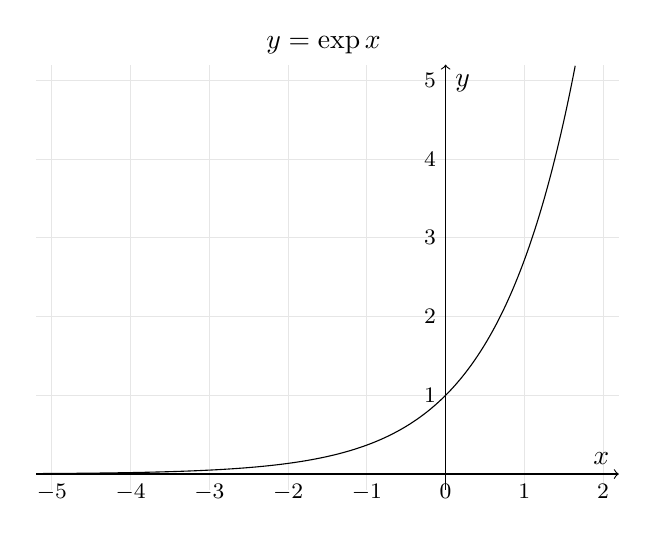
\begin{tikzpicture}\draw[color=gray,opacity=0.2] (-5.2,-0.2) grid(2.2,5.2); \draw[->] (-5.2, 0) -- (2.2, 0) node[above left]{$x$}; \draw[->] (0,-0.2) -- (0, 5.2) node[below right]{$y$}; \foreach \y in {1,...,5} \draw(0,\y) node[left]{\footnotesize$\y$}; \foreach \x in {-5,...,2} \draw(\x,0) node[below]{\footnotesize$\x$}; \draw[domain=-5.2:1.649, samples=1400, scale=1, smooth, variable=\x, black] plot (\x,{exp(\x)}); \node[above] at (current bounding box.north) {$y=\exp{x}$}; \end{tikzpicture}}{29/55}
\slideq{Courbe représentative de $\cos{x}$}{30/55}
\slider{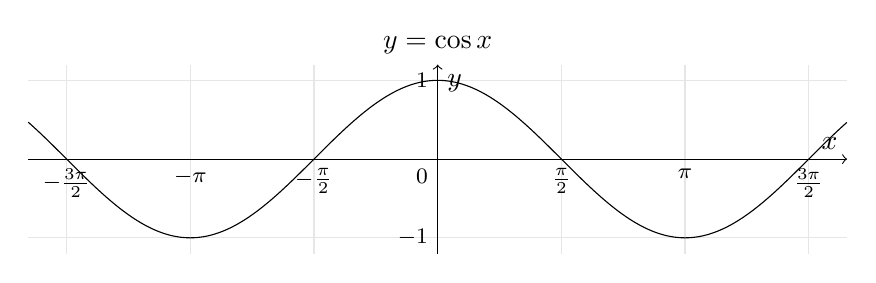
\begin{tikzpicture} \draw[color=gray,opacity=0.2] (-5.2,-1.2) grid[xstep=pi/2](5.2,1.2); \draw[->] (-5.2, 0) -- (5.2, 0) node[above left]{$x$}; \draw[->] (0,-1.2) -- (0, 1.2) node[below right]{$y$}; \foreach \y in {-1} \draw(0,\y) node[left]{\footnotesize$\y$}; \foreach \y in {1} \draw(0,\y) node[left]{\footnotesize$\y$}; \foreach \x[count=\cnt] in {-\frac{\pi}{2},-\pi,-\frac{3\pi}{2}} \draw({(-\cnt/2)*pi},0) node[below]{\footnotesize$\x$}; \foreach \x[count=\cnt] in {\frac{\pi}{2},\pi,\frac{3\pi}{2}} \draw({(\cnt/2)*pi},0) node[below]{\footnotesize$\x$}; \draw(0,0) node[below left]{\footnotesize$0$}; \draw[domain=-5.2:5.2, samples=1000, smooth, variable=\x, black] plot (\x, {cos(\x r)}); \node[above] at (current bounding box.north) {$y=\cos{x}$};\end{tikzpicture}}{30/55}
\slideq{Courbe représentative de $\tan{x}$}{31/55}
\slider{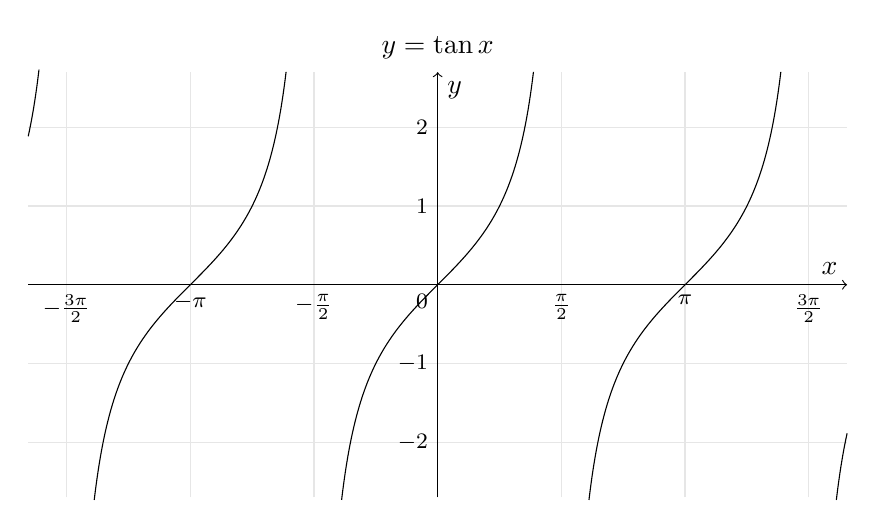
\begin{tikzpicture} \draw[color=gray,opacity=0.2] (-5.2,-2.7) grid[xstep=pi/2](5.2,2.7); \draw[->] (-5.2, 0) -- (5.2, 0) node[above left]{$x$}; \draw[->] (0,-2.7) -- (0, 2.7) node[below right]{$y$};  \foreach \y in {-2,-1} \draw(0,\y) node[left]{\footnotesize$\y$}; \foreach \y in {1,2} \draw(0,\y) node[left]{\footnotesize$\y$}; \foreach \x[count=\cnt] in {-\frac{\pi}{2},-\pi,-\frac{3\pi}{2}} \draw({(-\cnt/2)*pi},0) node[below]{\footnotesize$\x$}; \foreach \x[count=\cnt] in {\frac{\pi}{2},\pi,\frac{3\pi}{2}} \draw({(\cnt/2)*pi},0) node[below]{\footnotesize$\x$}; \draw(0,0) node[below left]{\footnotesize$0$}; \foreach \x in {-1,0,1} \draw[domain=\x*pi-1.22:\x*pi+1.22, samples=500, scale=1, smooth, variable=\x, black] plot (\x,{tan(\x r)}); \draw[domain=-5.2:-2*pi+1.22, samples=500, scale=1, smooth, variable=\x, black] plot (\x,{tan(\x r)}); \draw[domain=2*pi-1.22:5.2, samples=500, scale=1, smooth, variable=\x, black] plot (\x,{tan(\x r)}); \node[above] at (current bounding box.north) {$y=\tan{x}$}; \end{tikzpicture} }{31/55}
\slideq{$n\in\N^*$, $x\in\R$\linebreak$\der[n]{\ch{x}}$}{32/55}
\slider{$\left\{\begin{matrix*}[l]\ch{x}&\;\text{si }n\in2\N\\\sh{x}&\;\text{sinon}\end{matrix*}\right.\!$}{32/55}
\slideq{$\der{\ash{x}}$}{33/55}
\slider{$\frac{1}{\sqrt{x^2+1}}$}{33/55}
\slideq{$\lim{x\to0}{\frac{\ch{x}-1}{x^2}}$}{34/55}
\slider{$\frac{1}{2}$}{34/55}
\slideq{$\der{\tan{x}}$}{35/55}
\slider{$\frac{1}{\cos[2]{x}}=1+\tan[2]{x}$}{35/55}
\slideq{$\lim{x\to0}{\frac{\sh{x}}{x}}$}{36/55}
\slider{$1$}{36/55}
\slideq{Inégalités classiques de $\sin{x}$}{37/55}
\slider{$\forall x\in\R_+,\;\sin{x}\leqslant x$\linebreak$\forall x\in\R_-,\;\sin{x}\geqslant x$\linebreak$\forall x\in\R,\;\left|\sin{x}\right|\leqslant\left|x\right|$\linebreak$\forall x\in\left[0,\oldfrac{\pi}{2}\right],\;\sin{x}\geqslant\oldfrac{2x}{\pi}$}{37/55}
\slideq{Courbe représentative de $\acos{x}$}{38/55}
\slider{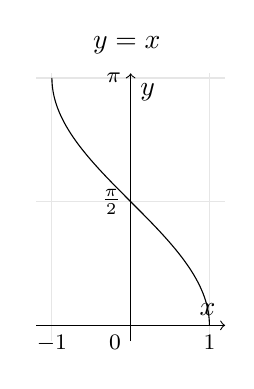
\begin{tikzpicture} \draw[color=gray,opacity=0.2] (-1.2,-0.2) grid[ystep=pi/2](1.2,3.2); \draw[->] (-1.2, 0) -- (1.2, 0) node[above left]{$x$}; \draw[->] (0,-0.2) -- (0, 3.2) node[below right]{$y$}; \foreach \y[count=\cnt] in {\frac{\pi}{2},\pi} \draw(0,{(\cnt/2)*pi}) node[left]{\footnotesize$\y$}; \foreach \x in {-1} \draw(\x,0) node[below]{\footnotesize$\x$}; \foreach \x in {1} \draw(\x,0) node[below]{\footnotesize$\x$}; \draw(0,0) node[below left]{\footnotesize$0$}; \draw[domain=pi:0, samples=400, scale=1, smooth, variable=\x, black] plot ({cos(\x r)},\x); \node[above] at (current bounding box.north) {$y=\acos{x}$}; \end{tikzpicture}}{38/55}
\slideq{Courbe représentative de $\ch{x}$}{39/55}
\slider{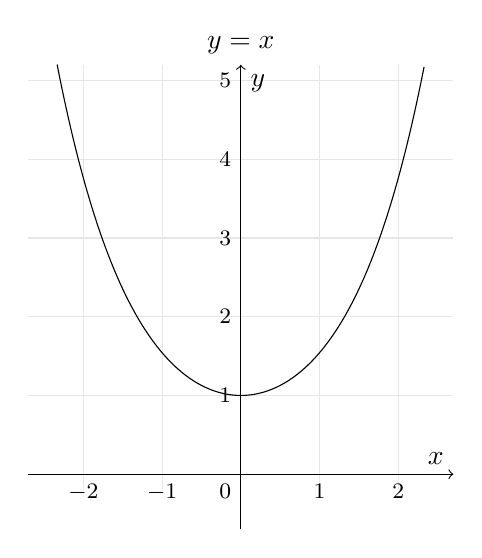
\begin{tikzpicture} \draw[color=gray,opacity=0.2] (-2.7,-0.2) grid (2.7,5.2); \draw[->] (-2.7, 0) -- (2.7, 0) node[above left]{$x$}; \draw[->] (0,-0.7) -- (0, 5.2) node[below right]{$y$}; \foreach \y in {1,...,5} \draw(0,\y) node[left]{\footnotesize$\y$}; \foreach \x in {-2,-1} \draw(\x,0) node[below]{\footnotesize$\x$}; \foreach \x in {1,2} \draw(\x,0) node[below]{\footnotesize$\x$}; \draw(0,0) node[below left]{\footnotesize$0$}; \draw[domain=-2.333:2.333, samples=500, scale=1, smooth, variable=\x, black] plot (\x,{(exp(\x)+exp(-\x))/2}); \node[above] at (current bounding box.north) {$y=\ch{x}$}; \end{tikzpicture}}{39/55}
\slideq{$\der{\atan{x}}$}{40/55}
\slider{$\frac{1}{1+x^2}$}{40/55}
\slideq{$\lim{x\to0}{\frac{\asin{x}}{x}}$}{41/55}
\slider{$1$}{41/55}
\slideq{$\lim{x\to0}{\frac{\tan{x}}{x}}$}{42/55}
\slider{$1$}{42/55}
\slideq{$\der{\ath{x}}$}{43/55}
\slider{$\frac{1}{1-x^2}$}{43/55}
\slideq{Courbe représentative de $\atan{x}$}{44/55}
\slider{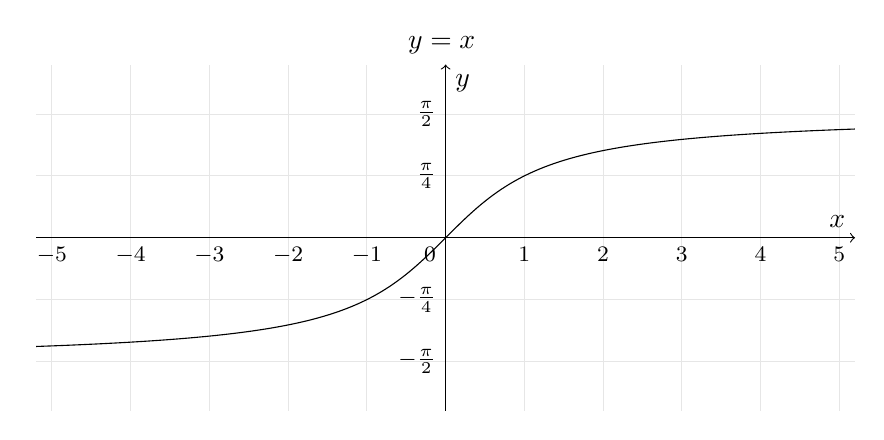
\begin{tikzpicture} \draw[color=gray,opacity=0.2] (-5.2,-2.2) grid[ystep=pi/4](5.2,2.2); \draw[->] (-5.2, 0) -- (5.2, 0) node[above left]{$x$}; \draw[->] (0,-2.2) -- (0, 2.2) node[below right]{$y$}; \foreach \y[count=\cnt] in {-\frac{\pi}{4},-\frac{\pi}{2}} \draw(0,{(-\cnt/4)*pi}) node[left]{\footnotesize$\y$}; \foreach \y[count=\cnt] in {\frac{\pi}{4},\frac{\pi}{2}} \draw(0,{(\cnt/4)*pi}) node[left]{\footnotesize$\y$}; \foreach \x in {-5,...,-1} \draw(\x,0) node[below]{\footnotesize$\x$}; \foreach \x in {1,...,5} \draw(\x,0) node[below]{\footnotesize$\x$}; \draw(0,0) node[below left]{\footnotesize$0$}; \draw[domain=-5.2:5.2, samples=2000, scale=1, smooth, variable=\x, black] plot (\x,{rad(atan(\x))}); \node[above] at (current bounding box.north) {$y=\atan{x}$}; \end{tikzpicture}}{44/55}
\slideq{Propriété remarquable de $\acos{x}$ et $\asin{x}$}{45/55}
\slider{$\acos{x}+\asin{x}=\frac{\pi}{2}$}{45/55}
\slideq{Courbe représentative de $\sin{x}$}{46/55}
\slider{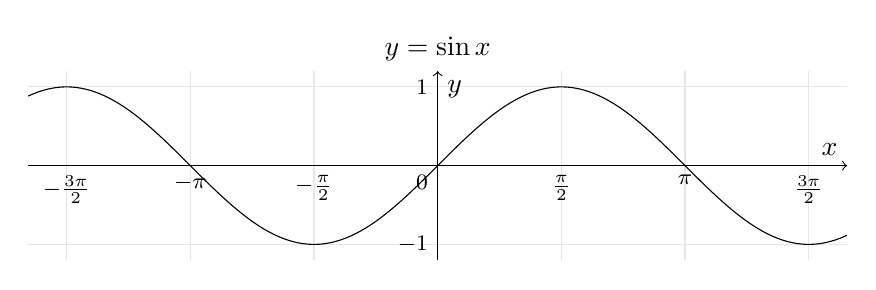
\begin{tikzpicture} \draw[color=gray,opacity=0.2] (-5.2,-1.2) grid[xstep=pi/2](5.2,1.2); \draw[->] (-5.2, 0) -- (5.2, 0) node[above left]{$x$}; \draw[->] (0,-1.2) -- (0, 1.2) node[below right]{$y$}; \foreach \y in {-1} \draw(0,\y) node[left]{\footnotesize$\y$}; \foreach \y in {1} \draw(0,\y) node[left]{\footnotesize$\y$}; \foreach \x[count=\cnt] in {-\frac{\pi}{2},-\pi,-\frac{3\pi}{2}} \draw({(-\cnt/2)*pi},0) node[below]{\footnotesize$\x$}; \foreach \x[count=\cnt] in {\frac{\pi}{2},\pi,\frac{3\pi}{2}} \draw({(\cnt/2)*pi},0) node[below]{\footnotesize$\x$}; \draw(0,0) node[below left]{\footnotesize$0$}; \draw[domain=-5.2:5.2, samples=1000, smooth, variable=\x, black] plot (\x, {sin(\x r)}); \node[above] at (current bounding box.north) {$y=\sin{x}$};\end{tikzpicture}}{46/55}
\slideq{Inégalités classiques de $\sh{x}$}{47/55}
\slider{$\forall x\in\R_+,\;\sh{x}\geqslant x$\linebreak$\forall x\in\R_-,\;\sh{x}\leqslant x$}{47/55}
\slideq{Propriétés remarquables de $\atan{x}$}{48/55}
\slider{$\forall x\in\R,\;\tan{\atan{x}}=x$\linebreak$\forall x\in\left]-\oldfrac{\pi}{2},\oldfrac{\pi}{2}\right[,\;\atan{\tan{x}}=x$\linebreak$\forall n\in\N,\;\forall x\in\left]-\oldfrac{\pi}{2}+n\pi,\oldfrac{\pi}{2}+n\pi\right[$\linebreak$\atan{\tan{x}}=x-n\pi$\linebreak$\forall x\in\R^*,\;\atan{x}+\atan{\oldfrac{1}{x}}=\oldfrac{x}{\left|x\right|}\oldfrac{\pi}{2}$}{48/55}
\slideq{Courbe représentative de $\ath{x}$}{49/55}
\slider{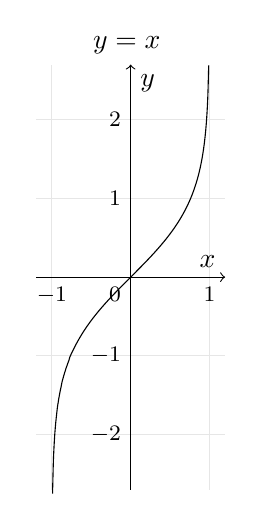
\begin{tikzpicture} \draw[color=gray,opacity=0.2] (-1.2,-2.7) grid (1.2,2.7); \draw[->] (-1.2, 0) -- (1.2, 0) node[above left]{$x$}; \draw[->] (0,-2.7) -- (0, 2.7) node[below right]{$y$}; \foreach \y in {-2,-1,1,2} \draw(0,\y) node[left]{\footnotesize$\y$}; \foreach \x in {-1} \draw(\x,0) node[below]{\footnotesize$\x$}; \foreach \x in {1} \draw(\x,0) node[below]{\footnotesize$\x$}; \draw(0,0) node[below left]{\footnotesize$0$}; \draw[domain=-0.992:0.992, samples=200, scale=1, smooth, variable=\x, black] plot (\x,{ln((1+\x)/(1-\x))/2}); \node[above] at (current bounding box.north) {$y=\ath{x}$}; \end{tikzpicture}}{49/55}
\slideq{Courbe représentative de $\th{x}$}{50/55}
\slider{\begin{tikzpicture} \draw[color=gray,opacity=0.2] (-5.2,-1.2) grid (5.2,1.2); \draw[->] (-5.2, 0) -- (5.2, 0) node[above left]{$x$}; \draw[->] (0,-1.2) -- (0, 1.2) node[below right]{$y$}; \foreach \y in {-1,1} \draw(0,\y) node[left]{\footnotesize$\y$}; \foreach \x in {-5,...,-1} \draw(\x,0) node[below]{\footnotesize$\x$}; \foreach \x in {1,...,5} \draw(\x,0) node[below]{\footnotesize$\x$}; \draw(0,0) node[below left]{\footnotesize$0$}; \draw[domain=-5.2:5.2, samples=1100, scale=1, smooth, variable=\x, black] plot (\x,{(exp(\x)-exp(-\x))/(exp(\x)+exp(-\x))}); \node[above] at (current bounding box.north) {$y=\th{x}$}; \end{tikzpicture}}{50/55}
\slideq{$n\in\N^*$, $x\in\R$\linebreak$\der[n]{\sin{x}}$}{51/55}
\slider{$\sin{x+\frac{n\pi}{2}}=\left\{\begin{matrix*}[l]\l-1\r^{\left\lfloor\oldfrac{n}{2}\right\rfloor}\sin{x}&\;\text{si }n\in2\N\\\l-1\r^{\left\lfloor\oldfrac{n}{2}\right\rfloor}\cos{x}&\;\text{sinon}\end{matrix*}\right.\!$}{51/55}
\slideq{Propriétés remarquables de $\asin{x}$}{52/55}
\slider{$\forall x\in\left[-1,1\right],\;\sin{\asin{x}}=x$\linebreak$\forall x\in\left[-\oldfrac{\pi}{2},\oldfrac{\pi}{2}\right],\;\asin{\sin{x}}=x$\linebreak$\forall x\in\left[\oldfrac{\pi}{2},\oldfrac{3\pi}{2}\right],\;\asin{\sin{x}}=\pi-x$}{52/55}
\slideq{$\der{\ach{x}}$}{53/55}
\slider{$\frac{1}{\sqrt{x^2-1}}$}{53/55}
\slideq{Courbe représentative de $\ach{x}$}{54/55}
\slider{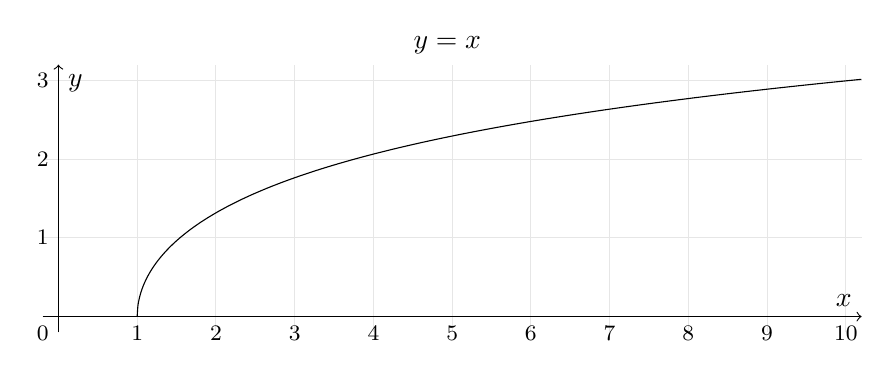
\begin{tikzpicture} \draw[color=gray,opacity=0.2] (-0.2,-0.2) grid (10.2,3.2); \draw[->] (-0.2, 0) -- (10.2, 0) node[above left]{$x$}; \draw[->] (0,-0.2) -- (0, 3.2) node[below right]{$y$}; \foreach \y in {1,...,3} \draw(0,\y) node[left]{\footnotesize$\y$}; \foreach \x in {1,...,10} \draw(\x,0) node[below]{\footnotesize$\x$}; \draw(0,0) node[below left]{\footnotesize$0$}; \draw[domain=1:10.2, samples=1100, scale=1, smooth, variable=\x, black] plot (\x,{ln(\x+sqrt(\x*\x-1))}); \node[above] at (current bounding box.north) {$y=\ach{x}$}; \end{tikzpicture}}{54/55}
\slideq{$\lim{x\to0}{\frac{1-\cos{x}}{x^2}}$}{55/55}
\slider{$\frac{1}{2}$}{55/55}
\end{document}